%%%%% Code to convert a Tikz picutre to a standalone picutre file %%%%%
%%%%% See for more information: https://hh360.user.srcf.net/blog/2015/04/converting-from-tikz-to-png/ %%%%%
% Example command for PNG creation: pdflatex --shell-escape Tikz_picture_to_PNG.tex
\documentclass[preview,border=4mm,convert={density=600,outext=.png}]{standalone}

\usepackage{url}
\usepackage{tikz}
\usepackage{color}
\begin{document}

% Make a white background for the full document. This is necessary, because the default case for a PNG picture is a alpha 255 background
\pagecolor{white}

% Prepare internationalization for the strings in the picture
% See: https://tex.stackexchange.com/questions/60781/managing-multiple-translation-of-a-single-document
\newif\ifen
\newif\ifde
\newcommand{\en}[1]{\ifen#1\fi}
\newcommand{\de}[1]{\ifde#1\fi}

% English:
%\entrue
% German:
\detrue

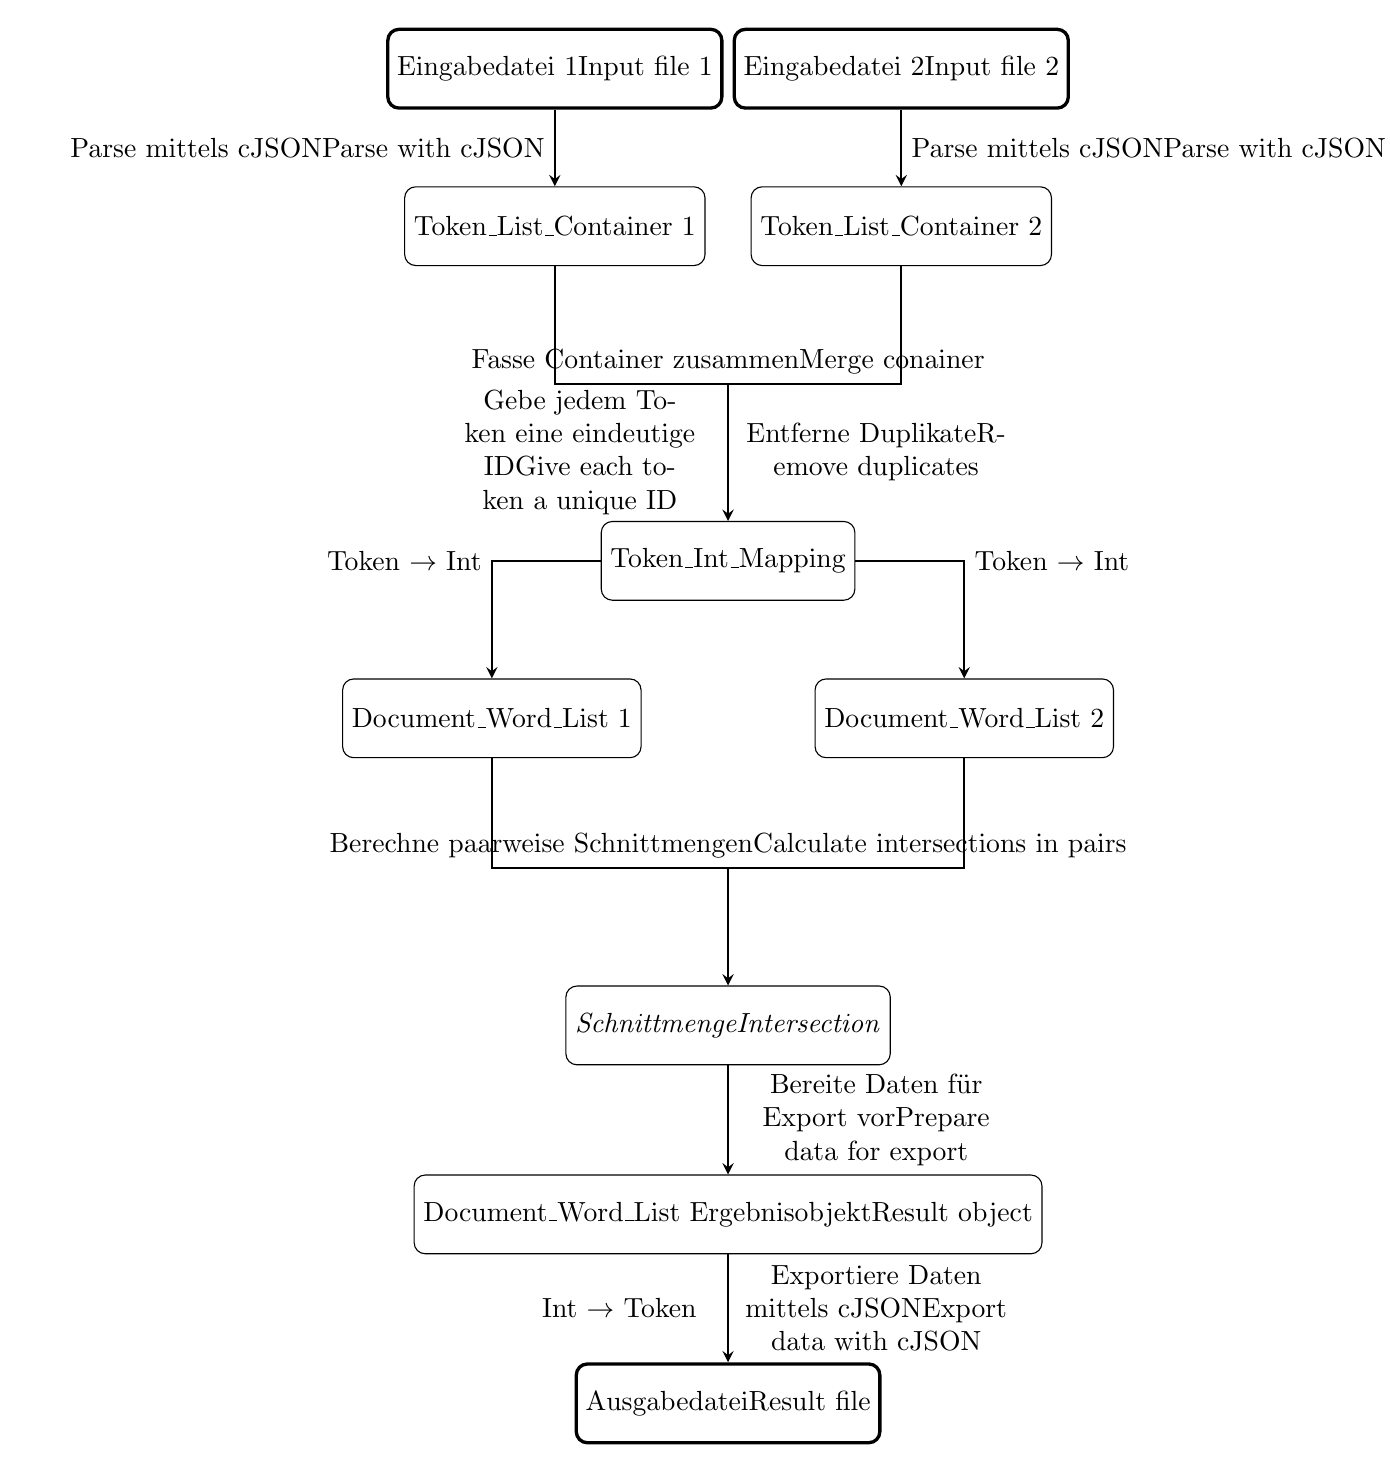
\begin{tikzpicture}[node distance=2cm]
    % Centering the picutre (This value maybe need to be adjusted, when the picutre was changed)
    \hspace*{0.425cm}

    \tikzstyle{in_out} = [rectangle, rounded corners, minimum width=3cm, minimum height=1cm, text centered, draw=black, very thick]%, fill=red!30]
    \tikzstyle{rect} = [rectangle, rounded corners, minimum width=3cm, minimum height=1cm, text centered, draw=black]
    \tikzstyle{process} = [rectangle, rounded corners, minimum width=0.75cm, minimum height=0.75cm,text centered, draw=black, fill=gray!12.5]
    \tikzstyle{intersection} = [rectangle, rounded corners, minimum width=4cm, minimum height=1cm, text centered, draw=black]
    \tikzstyle{arrow} = [thick,->,>=stealth]

            % node[Optionen](Name){Inhalt}
            \node (Eingabedatei1) [in_out, xshift=0cm] {\de{Eingabedatei 1}\en{Input file 1}};
            \node (Eingabedatei2) [in_out, xshift=4.4cm] {\de{Eingabedatei 2}\en{Input file 2}};

            \node (Token_List_Container1) [rect, below of=Eingabedatei1] {Token\_List\_Container 1};
            \node (Token_List_Container2) [rect, below of=Eingabedatei2] {Token\_List\_Container 2};

            \node (Inv1) [coordinate, below of=Token_List_Container1, xshift=2.2cm, yshift=-0cm, label=\de{Fasse Container zusammen}\en{Merge conainer}] {};

            \node (Token_Int_Mapping) [rect, below of=Inv1, yshift=-0.25cm] {Token\_Int\_Mapping};
            \node (Document_Word_List1) [rect, below of=Token_Int_Mapping, xshift=-3cm] {Document\_Word\_List 1};
            \node (Document_Word_List2) [rect, below of=Token_Int_Mapping, xshift=3cm] {Document\_Word\_List 2};

            \node (Inv2) [coordinate, below of=Document_Word_List1, xshift=3cm, yshift=0.1cm, label=\de{Berechne paarweise Schnittmengen}\en{Calculate intersections in pairs}] {};
            \node (Intersection) [intersection, below of=Inv2, yshift=0.0cm] {\emph{\de{Schnittmenge}\en{Intersection}}};
            \node (Document_Word_List_Ergebnis) [rect, below of=Intersection, yshift=-0.4cm] {Document\_Word\_List \de{Ergebnisobjekt}\en{Result object}};

            \node (Ausgabedatei) [in_out, below of=Document_Word_List_Ergebnis, yshift=-0.4cm] {\de{Ausgabedatei}\en{Result file}};

            % ----- ----- ----- ----- ----- ----- ----- ----- ----- ----- ----- ----- ----- ----- ----- ----- ----- ----- -----

            \draw [arrow] (Eingabedatei1) -- node[anchor=east] {\de{Parse mittels cJSON}\en{Parse with cJSON}} (Token_List_Container1);
            \draw [arrow] (Eingabedatei2) -- node[anchor=west] {\de{Parse mittels cJSON}\en{Parse with cJSON}} (Token_List_Container2);
            \draw [thick] (Token_List_Container1) |- (Inv1);
            \draw [thick] (Token_List_Container2) |- (Inv1);
            \draw [arrow] (Inv1) -- node[anchor=west, text centered, text width=3.5cm]{\de{Entferne Duplikate}\en{Remove duplicates}} node[anchor=east, text centered, text width=3.5cm]{\de{Gebe jedem Token eine eindeutige ID}\en{Give each token a unique ID}} (Token_Int_Mapping);
            \draw [arrow] (Token_Int_Mapping) -| node[anchor=east] {Token $ \rightarrow $ Int} (Document_Word_List1);
            \draw [arrow] (Token_Int_Mapping) -| node[anchor=west] {Token $ \rightarrow $ Int} (Document_Word_List2);
            \draw [thick] (Document_Word_List1) |- (Inv2);
            \draw [thick] (Document_Word_List2) |- (Inv2);
            \draw [arrow] (Inv2) -- (Intersection);
            \draw [arrow] (Intersection) -- node[anchor=west, text centered, text width=3.5cm] {\de{Bereite Daten für Export vor}\en{Prepare data for export}} (Document_Word_List_Ergebnis);
            \draw [arrow] (Document_Word_List_Ergebnis) -- node[anchor=east, text centered, text width=2.5cm] {Int $ \rightarrow $ Token} node[anchor=west, text centered, text width=3.5cm] {\de{Exportiere Daten mittels cJSON}\en{Export data with cJSON}} (Ausgabedatei);
\end{tikzpicture}

\end{document}
